\documentclass[aspectratio=169]{beamer}

% Shared Beamer settings for Applied Machine Learning lectures (UPES).
% Keep this file free of \documentclass to allow reuse via \input.

% Allow lecture sources to use shared theme/assets without copying them into each lecture folder.
% NOTE: These paths are relative to `Unit-xx/Lecture-yy/latex/` (and `Lab/Experiment-xx/latex/`).
\makeatletter
\def\input@path{{../../../_shared/}{../../../_shared/UPES-Beamer-Theme/}}
\makeatother

\usetheme{UPES}
\setbeamertemplate{navigation symbols}{}

\usepackage{amsmath}
\usepackage{amssymb}
\usepackage{booktabs}
\usepackage{graphicx}
\usepackage{hyperref}
\usepackage{xcolor}
\usepackage{listings}

% Code listings (Python-oriented for this subject).
\lstset{
  language=Python,
  basicstyle=\ttfamily\small,
  keywordstyle=\color{blue},
  commentstyle=\color{gray},
  stringstyle=\color{teal},
  showstringspaces=false,
  columns=fullflexible,
  breaklines=true
}

\usepackage{tikz}
\usetikzlibrary{arrows.meta,positioning,shapes.geometric,calc,fit,backgrounds}

% Per-slide source line (references shown on the slide itself).
\newcommand{\slidesources}[1]{%
  \vfill
  {\tiny\color{gray}\raggedright\sloppy\parbox{\linewidth}{Sources: #1}\par}%
}

% Unit-wise source strings for this subject (used by slides/notes).
% Path is relative to the lecture `latex/` folder (the compilation CWD).
% Source strings for Applied Machine Learning (CSAI2017P) — used by slides + notes.
% Prescribed texts and reference books are taken from the course syllabus.
% Support texts are the author-hosted open-access editions:
%   statlearning.com            (ISL with Python)
%   probml.github.io/pml-book   (Murphy, Probabilistic Machine Learning)
%   d2l.ai                      (Dive into Deep Learning)
%   mml-book.github.io          (Mathematics for Machine Learning)

\newcommand{\AMLRepoURL}{https://github.com/tali7c/Applied-Machine-Learning}

% --- prescribed -------------------------------------------------------------
\newcommand{\AMLPrescribed}{%
M\"uller and Guido, \textit{Introduction to Machine Learning with Python}, O'Reilly, 2016.;%
Bishop, \textit{Pattern Recognition and Machine Learning}, Springer, 2006.;%
Murphy, \textit{Machine Learning: A Probabilistic Perspective}, MIT Press, 2012.;%
Han, Kamber and Pei, \textit{Data Mining: Concepts and Techniques} (3e), Morgan Kaufmann, 2012.%
}

% --- unit-wise ---------------------------------------------------------------
\newcommand{\AMLUnitISources}{%
M\"uller and Guido, \textit{Introduction to Machine Learning with Python}, Ch. 1.;%
Bishop, \textit{Pattern Recognition and Machine Learning}, Ch. 1.;%
Murphy, \textit{Probabilistic Machine Learning: An Introduction}, MIT Press, 2022, Ch. 1.;%
Mitchell, \textit{Machine Learning}, McGraw Hill, 1997, Ch. 1.;%
Scikit-learn documentation, accessed 2026-08-04.%
}

\newcommand{\AMLUnitIISources}{%
Bishop, \textit{Pattern Recognition and Machine Learning}, \S1.5, \S4.3, \S7.1.;%
Zhang, Lipton, Li and Smola, \textit{Dive into Deep Learning}, \S3.4.;%
Shalev-Shwartz and Ben-David, \textit{Understanding Machine Learning}, Ch. 15.;%
Murphy, \textit{Probabilistic Machine Learning: An Introduction}, Ch. 5.%
}

\newcommand{\AMLUnitIIISources}{%
Zhang, Lipton, Li and Smola, \textit{Dive into Deep Learning}, Ch. 12 (Optimization Algorithms).;%
Deisenroth, Faisal and Ong, \textit{Mathematics for Machine Learning}, Ch. 7.;%
Kingma and Ba, ``Adam: A Method for Stochastic Optimization,'' ICLR 2015.;%
Ruder, ``An overview of gradient descent optimization algorithms,'' arXiv:1609.04747, 2016.%
}

\newcommand{\AMLUnitIVSources}{%
Han, Kamber and Pei, \textit{Data Mining: Concepts and Techniques} (3e), Ch. 3.;%
M\"uller and Guido, \textit{Introduction to Machine Learning with Python}, Ch. 3--4.;%
James, Witten, Hastie, Tibshirani and Taylor, \textit{An Introduction to Statistical Learning with Python}, Ch. 5--6, 12.;%
Scikit-learn documentation (preprocessing, model selection), accessed 2026-08-04.%
}

\newcommand{\AMLUnitVSources}{%
James et al., \textit{An Introduction to Statistical Learning with Python}, Ch. 3--6.;%
Bishop, \textit{Pattern Recognition and Machine Learning}, Ch. 3.;%
Deisenroth, Faisal and Ong, \textit{Mathematics for Machine Learning}, Ch. 9.;%
M\"uller and Guido, \textit{Introduction to Machine Learning with Python}, \S2.3.%
}

\newcommand{\AMLUnitVISources}{%
Han, Kamber and Pei, \textit{Data Mining: Concepts and Techniques} (3e), Ch. 8--9.;%
James et al., \textit{An Introduction to Statistical Learning with Python}, Ch. 8--9.;%
Bishop, \textit{Pattern Recognition and Machine Learning}, Ch. 4--5, 7, 14.;%
Zhang et al., \textit{Dive into Deep Learning}, Ch. 5.%
}

\newcommand{\AMLUnitVIISources}{%
Han, Kamber and Pei, \textit{Data Mining: Concepts and Techniques} (3e), Ch. 10.;%
James et al., \textit{An Introduction to Statistical Learning with Python}, Ch. 12.;%
M\"uller and Guido, \textit{Introduction to Machine Learning with Python}, \S3.5.;%
Ester, Kriegel, Sander and Xu, ``A density-based algorithm for discovering clusters (DBSCAN),'' KDD 1996.%
}

\newcommand{\AMLLabSources}{%
M\"uller and Guido, \textit{Introduction to Machine Learning with Python}, companion notebooks.;%
McKinney, \textit{Python for Data Analysis} (3e), O'Reilly, 2022.;%
Scikit-learn user guide, accessed 2026-08-04.;%
Matplotlib and Seaborn documentation, accessed 2026-08-04.%
}



\graphicspath{{../figures/}{../images/}{../../../_shared/}{../../../_shared/UPES-Beamer-Theme/}}

\title[Applied Machine Learning]{Applied Machine Learning}
\subtitle{Unit 05 -- Lecture 12: Regularization -- Ridge and Lasso}
\author{Tofik Ali}
\institute{School of Computer Science, UPES Dehradun}
\date{Autumn 2026}

% ---- a compact "output" block so code and its result sit together ----------
\lstdefinestyle{outblk}{
  basicstyle=\ttfamily\scriptsize\color{black!75},
  backgroundcolor=\color{black!5}, frame=leftline, framerule=2pt,
  rulecolor=\color{black!30}, breaklines=true, columns=fullflexible,
  keepspaces=true,   % several outputs below are aligned tables
  language={},       % printed output is not Python: do not syntax-highlight it
  xleftmargin=4pt, aboveskip=1pt, belowskip=1pt, literate={-}{{-}}1}
\lstnewenvironment{outblk}{\lstset{style=outblk}}{}

\begin{document}

\UPESCoverFrame
\setcounter{framenumber}{0}

\begin{frame}
  \titlepage
  \begin{center}
    \footnotesize Ridge, lasso, elastic net, and how to choose the penalty\\[0.25em]
    \footnotesize Topic focus: \textbf{deliberately fitting the training data
    worse, on purpose}\\[0.25em]
    \footnotesize Repository: \texttt{\AMLRepoURL}
  \end{center}
  \slidesources{\AMLUnitVSources}
\end{frame}

\begin{frame}{Quick Links}
  \centering
  \hyperlink{sec:why}{\beamerbutton{Why}}\hspace{0.35em}
  \hyperlink{sec:ridge}{\beamerbutton{Ridge}}\hspace{0.35em}
  \hyperlink{sec:lasso}{\beamerbutton{Lasso}}\hspace{0.35em}
  \hyperlink{sec:paths}{\beamerbutton{Paths}}\hspace{0.35em}
  \hyperlink{sec:scale}{\beamerbutton{Scaling}}\hspace{0.35em}
  \hyperlink{sec:cv}{\beamerbutton{Choosing $\lambda$}}\hspace{0.35em}
  \hyperlink{sec:bv}{\beamerbutton{Bias--variance}}\hspace{0.35em}
  \hyperlink{sec:enet}{\beamerbutton{Elastic net}}\hspace{0.35em}
  \hyperlink{sec:summary}{\beamerbutton{Summary}}
\end{frame}

\begin{frame}{Agenda}
  \tableofcontents
\end{frame}

\begin{frame}[shrink=6]{How this lecture works}
  \begin{columns}[T]
    \begin{column}{0.48\textwidth}
      \begin{block}{Every idea appears twice}
        \begin{enumerate}
          \item \textbf{By hand} --- three numbers, a $2\times2$ inverse, four
            OLS coefficients. Small enough to check on paper.
          \item \textbf{In code} --- the same arithmetic on real data, so you
            see that \texttt{Ridge} and \texttt{Lasso} do exactly that and
            nothing more.
        \end{enumerate}
      \end{block}
    \end{column}
    \begin{column}{0.48\textwidth}
      \begin{alertblock}{Commit before you look}
        Four slides ask you to predict a number before it is revealed. Write
        your guess down. Being wrong on paper is how the idea sticks.
      \end{alertblock}
    \end{column}
  \end{columns}
  \vspace{0.4em}
  \begin{center}
    \small The centrepiece is \textbf{one figure}: ten coefficient curves
    under each penalty. Ridge decays them smoothly and never reaches zero;
    lasso kills them one at a time.
  \end{center}
\end{frame}

\begin{frame}{One dataset, one seed}
  \begin{columns}[T]
    \begin{column}{0.48\textwidth}
      \begin{block}{The data}
        \small scikit-learn's bundled \texttt{load\_diabetes}, in both its
        pre-scaled and its original-units form. Everything else is synthetic,
        drawn from the same seed. Nothing is downloaded.
      \end{block}
    \end{column}
    \begin{column}{0.48\textwidth}
      \begin{block}{The randomness}
        \small One seed for the whole lecture:
        \texttt{np.random.default\_rng(0)} and \texttt{random\_state=0}.
        Every listing that draws, splits or resamples shows it. Where the
        \emph{spread} is the point --- twenty $p>n$ draws, thirty bootstrap
        resamples --- the seeds are $0, 1, 2, \dots$, derived from that one.
      \end{block}
    \end{column}
  \end{columns}
  \vspace{0.5em}
  \begin{exampleblock}{Why this matters to you}
    \centering\small
    Every number in this deck is printed by one script. Run the code as
    written and you get the same numbers --- which is the only reason to
    believe a number on a slide.
  \end{exampleblock}
\end{frame}

% =====================================================================
\section[Why]{The problem regularization solves}
\label{sec:why}

\begin{frame}[shrink=8]{Where we are: three failures, one cure}
  \begin{center}\small
  \begin{tabular}{@{}lp{4.4cm}p{4.6cm}@{}}
    \toprule
    \textbf{Unit V raised} & \textbf{What goes wrong} & \textbf{What the
      penalty does}\\
    \midrule
    \textbf{Over-fitting} & the fitted surface chases the noise; huge
      $\|\beta\|$ & caps $\|\beta\|$, so the surface cannot wiggle\\[4pt]
    \textbf{Multicollinearity} & $X^{\!\top}\!X$ nearly singular; coefficients
      huge, of opposite sign, unstable & adds $\lambda$ to the diagonal, so
      the matrix is well conditioned again\\[4pt]
    \textbf{Perfect separation} & the logistic likelihood has no maximum;
      $\|\beta\| \to \infty$ & the penalty is the only thing stopping it\\
    \bottomrule
  \end{tabular}
  \end{center}
  \vspace{0.2em}
  \begin{block}{Stop asking for the smallest training error}
    \[
      \hat\beta \;=\; \arg\min_\beta\ \underbrace{\text{loss}(\beta)}_{\text{fit
      the data}} \;+\; \lambda\,\underbrace{\text{pen}(\beta)}_{\text{stay
      small}}
    \]
    \small $\lambda = 0$ gives back the unpenalised fit; $\lambda \to \infty$
    gives the constant model. Everything interesting is in between --- and
    $\lambda$ is \textbf{not fitted}, it is chosen by cross-validation, which
    is why this lecture could not come before the validation material.
  \end{block}
\end{frame}

\begin{frame}[fragile,shrink=8]{Predict first \#1}
$n = 40$ rows, $p = 38$ columns of pure noise, and only \emph{three} of them
carry any signal at all. Fit ordinary least squares. Then fit ridge with
$\alpha = 10$.

\begin{center}
  \textbf{What does each score on $2000$ fresh rows?}
\end{center}
\vspace{0.2em}
\onslide<2->
\begin{outblk}
(a) over-fitting     n=40  p=38
    OLS   train R2 +0.9997   test R2 +0.1470   ||beta||    5.075
    ridge train R2 +0.9336   test R2 +0.6598   ||beta||    2.432
\end{outblk}
\onslide<3->
\begin{alertblock}{Ridge fits the training data \emph{worse}, on purpose}
  \footnotesize Training $R^2$ falls from $0.9997$ to $0.9336$ --- and test
  $R^2$ rises from $0.1470$ to $\mathbf{0.6598}$, a factor of four and a half.
  The coefficient vector halves in length. \textbf{Every point of training fit
  given up bought several points of test fit.}
\end{alertblock}
\end{frame}

\begin{frame}[fragile,shrink=8]{Multicollinearity: the coefficients will not stand still}
Two columns with $\mathrm{corr} = 0.99989$; the truth is $y = 2z$.
\begin{outblk}
(b) multicollinearity  corr(x1,x2) = 0.999885
    OLS   coefficients [ 6.5628 -4.54  ]
    ridge coefficients [1.0549 0.9486]
    the same fit on five bootstrap resamples of the same 100 rows:
       OLS [+11.0217,  -8.9539]   sum +2.0677      ridge [+1.1020, +0.9276]   sum +2.0297
       OLS [ +2.7446,  -0.6954]   sum +2.0492      ridge [+1.0332, +0.9985]   sum +2.0317
       OLS [ +6.7951,  -4.7408]   sum +2.0543      ridge [+1.0785, +0.9529]   sum +2.0315
       OLS [ +5.0355,  -3.0251]   sum +2.0105      ridge [+1.0354, +0.9583]   sum +1.9937
       OLS [ +7.5289,  -5.5234]   sum +2.0055      ridge [+1.0785, +0.9294]   sum +1.9867
\end{outblk}
\onslide<2->
\begin{alertblock}{Look down the two ``sum'' columns, then at the pairs}
  \footnotesize The \emph{sum} is stable in both --- always about $2.0$,
  because that is what the data determines. The \emph{split} is not: OLS puts
  $+11.0$ on one column and $-9.0$ on the other in the first resample and
  $+2.7 / -0.7$ in the second. \textbf{Ridge splits it evenly every time.}
\end{alertblock}
\end{frame}

\begin{frame}[fragile,shrink=6]{And the L10 case: perfect separation}
Six points, one feature, the classes perfectly separated. The maximum
likelihood estimate does not exist --- the slope runs away.
\begin{outblk}
(c) perfect separation, 6 points, one feature
    C = 1e+10     penalty strength 1/C = 1e-10     fitted slope     8.3469
    C = 1         penalty strength 1/C = 1         fitted slope     1.1043
    C = 0.01      penalty strength 1/C = 100       fitted slope     0.0561
\end{outblk}
\onslide<2->
\begin{center}\small
  \texttt{LogisticRegression} in scikit-learn is \textbf{L2-penalised by
  default}, with $C = 1$, and $C$ is $1/\lambda$. You have been using
  regularization since L10 without being told.
\end{center}
\onslide<3->
\begin{center}\small
  Turn the penalty off (\texttt{C}$\,=10^{10}$) and the slope climbs to $8.35$
  and would keep climbing with more iterations. \textbf{The penalty is what
  makes the answer exist.}
\end{center}
\end{frame}

% =====================================================================
\section[Ridge]{Ridge regression}
\label{sec:ridge}

\begin{frame}[shrink=6]{Ridge: the objective, two ways of writing it}
  \begin{exampleblock}{Penalised form}
    \[
      J(\beta) \;=\; \underbrace{(y - X\beta)^{\!\top}(y - X\beta)}_{\text{RSS}}
      \;+\; \lambda\,\beta^{\!\top}\beta ,
      \qquad \lambda \ge 0 .
    \]
  \end{exampleblock}
  \begin{exampleblock}{Constrained form --- the same problem}
    \[
      \min_\beta\ (y - X\beta)^{\!\top}(y - X\beta)
      \quad\text{subject to}\quad \|\beta\|_2^2 \le s .
    \]
  \end{exampleblock}
  \vspace{0.2em}
  \begin{block}{Two things to fix in your head now}
    \small \textbf{The intercept is not penalised.} $\beta_0$ is excluded from
    the sum; otherwise the model could not even represent a constant shift
    in $y$.\\[0.25em]
    \textbf{$\lambda$ is not a parameter.} It is a hyper-parameter: it is not
    estimated from the data by the fit, it is chosen from outside by
    cross-validation.
  \end{block}
\end{frame}

\begin{frame}[shrink=4]{Deriving the closed form --- four lines}
  Differentiate. $\dfrac{\partial}{\partial\beta}(y-X\beta)^{\!\top}(y-X\beta)
  = -2X^{\!\top}(y - X\beta)$ and
  $\dfrac{\partial}{\partial\beta}\lambda\beta^{\!\top}\beta = 2\lambda\beta$.
  \begin{align*}
    \nabla J(\beta) &= -2X^{\!\top}(y - X\beta) + 2\lambda\beta = 0\\[2pt]
    \Longrightarrow\quad X^{\!\top}y &= X^{\!\top}\!X\beta + \lambda\beta
      \;=\; (X^{\!\top}\!X + \lambda I)\,\beta\\[2pt]
    \Longrightarrow\quad
    \boxed{\ \hat\beta^{\,\mathrm{ridge}}
      = (X^{\!\top}\!X + \lambda I)^{-1} X^{\!\top}y\ }
  \end{align*}
  \begin{block}{Set $\lambda = 0$ and you get least squares back}
    \small $\hat\beta^{\,\mathrm{OLS}} = (X^{\!\top}\!X)^{-1}X^{\!\top}y$, the
    L8 formula. Ridge is one extra term on the diagonal --- and that one term
    is the whole lecture.
  \end{block}
  \begin{center}\small
    The Hessian is $2(X^{\!\top}\!X + \lambda I)$, which we are about to show
    is positive definite, so the stationary point is the unique minimum.
  \end{center}
\end{frame}

\begin{frame}[shrink=6]{The structural point: the inverse always exists}
  \begin{block}{Claim}
    For every $\lambda > 0$, the matrix $X^{\!\top}\!X + \lambda I$ is
    positive definite, and therefore invertible --- \textbf{whatever $X$ is}.
  \end{block}
  \begin{block}{Proof, one line}
    For any $v \ne 0$,
    \[
      v^{\!\top}(X^{\!\top}\!X + \lambda I)v
      \;=\; \|Xv\|^2 + \lambda\|v\|^2 \;\ge\; \lambda\|v\|^2 \;>\; 0 .
    \]
    \small The first term can be zero --- that is exactly what a singular
    $X^{\!\top}\!X$ means --- but the second cannot.
  \end{block}
  \begin{exampleblock}{The same thing in eigenvalues}
    \small If $X^{\!\top}\!X$ has eigenvalues $d_1^2 \ge \dots \ge d_p^2 \ge 0$,
    then $X^{\!\top}\!X + \lambda I$ has eigenvalues $d_j^2 + \lambda$, all
    strictly positive. \textbf{Adding $\lambda$ to the diagonal lifts every
    eigenvalue off the floor.}
  \end{exampleblock}
  \begin{center}\small
    So ridge has an answer in cases where \emph{ordinary least squares does
    not exist at all}. That is not a refinement; it is a change of kind.
  \end{center}
\end{frame}

\begin{frame}[fragile,shrink=10]{By hand \#1: three numbers, one feature}
  $x = (1, 2, 2)$, $y = (2, 3, 5)$, no intercept. Then
  $X^{\!\top}\!X = 1 + 4 + 4 = 9$ and $X^{\!\top}y = 2 + 6 + 10 = 18$, so
  \[
    \hat\beta(\lambda) \;=\; \frac{18}{9 + \lambda}
    \;=\; \underbrace{2}_{\hat\beta^{\mathrm{OLS}}}
      \times \underbrace{\frac{9}{9+\lambda}}_{\text{shrinkage factor}} .
  \]
\begin{lstlisting}
for lam in (0., 1., 9., 81.):
    print(Ridge(alpha=lam, fit_intercept=False).fit(x.reshape(-1,1), y).coef_)
\end{lstlisting}
\begin{outblk}
  lambda     0   beta = 18 / ( 9 +  0) = 2.0000   shrinkage factor 1.0000   sklearn 2.0000
  lambda     1   beta = 18 / ( 9 +  1) = 1.8000   shrinkage factor 0.9000   sklearn 1.8000
  lambda     9   beta = 18 / ( 9 +  9) = 1.0000   shrinkage factor 0.5000   sklearn 1.0000
  lambda    81   beta = 18 / ( 9 + 81) = 0.2000   shrinkage factor 0.1000   sklearn 0.2000
\end{outblk}
\onslide<2->
\begin{alertblock}{At $\lambda = X^{\!\top}\!X$ the coefficient is exactly halved}
  \footnotesize Four digits, four matches: \texttt{Ridge} is
  $(X^{\!\top}\!X+\lambda I)^{-1}X^{\!\top}y$ and nothing else. And note that
  $\lambda$ is measured \textbf{on the same scale as $X^{\!\top}\!X$} ---
  whether $9$ is ``a lot'' depends entirely on the size of the numbers in
  $X$, which is why Section~\ref{sec:scale} exists.
\end{alertblock}
\end{frame}

\begin{frame}[shrink=8]{Drawn: the minimum slides towards the origin}
  \begin{center}
    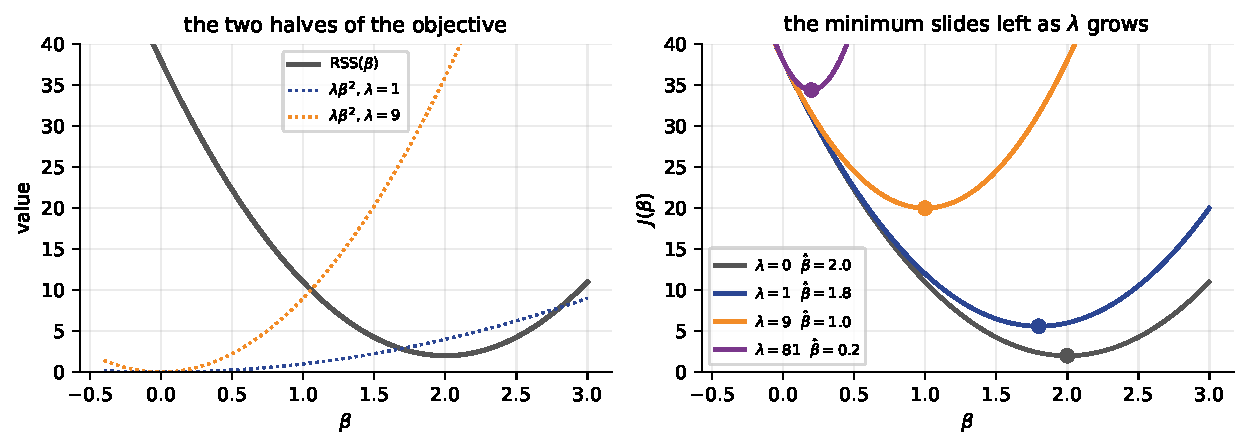
\includegraphics[width=0.86\textwidth]{handridge.pdf}
  \end{center}
  \begin{center}\small
    Left: RSS is a parabola with its minimum at $2$; $\lambda\beta^2$ is a
    parabola with its minimum at $0$. Right: their sum, for four values of
    $\lambda$. \textbf{Adding a bowl centred at the origin drags the minimum
    towards the origin, and never past it.}
  \end{center}
\end{frame}

\begin{frame}[shrink=8]{By hand \#2: a $2\times2$ inverse}
  $X = \left(\begin{smallmatrix}1&0\\0&1\\1&1\end{smallmatrix}\right)$,
  $y = (1,2,3)^{\!\top}$. Then
  $X^{\!\top}\!X = \left(\begin{smallmatrix}2&1\\1&2\end{smallmatrix}\right)$ and
  $X^{\!\top}y = (4,5)^{\!\top}$.
  \begin{center}\small
  \begin{tabular}{@{}lccrr@{}}
    \toprule
    $\lambda$ & $X^{\!\top}\!X + \lambda I$ & $\det$ & $\hat\beta$
      & $\|\hat\beta\|_2$\\
    \midrule
    $0$ & $\left(\begin{smallmatrix}2&1\\1&2\end{smallmatrix}\right)$ & $3$
      & $(1.0000,\ 2.0000)$ & $2.2361$\\[4pt]
    $1$ & $\left(\begin{smallmatrix}3&1\\1&3\end{smallmatrix}\right)$ & $8$
      & $(0.8750,\ 1.3750)$ & $1.6298$\\[4pt]
    $3$ & $\left(\begin{smallmatrix}5&1\\1&5\end{smallmatrix}\right)$ & $24$
      & $(0.6250,\ 0.8750)$ & $1.0753$\\
    \bottomrule
  \end{tabular}
  \end{center}
  \vspace{0.1em}
  Check the $\lambda=1$ row by hand:
  $\frac{1}{8}\left(\begin{smallmatrix}3&-1\\-1&3\end{smallmatrix}\right)
  \left(\begin{smallmatrix}4\\5\end{smallmatrix}\right)
  = \frac{1}{8}\left(\begin{smallmatrix}7\\11\end{smallmatrix}\right)
  = (0.875,\ 1.375)$.
  \begin{block}{Notice they do not shrink at the same rate}
    \small $\beta_1$ falls $12.5\%$ then a further $29\%$; $\beta_2$ falls
    $31\%$ then a further $36\%$. \textbf{Ridge is not a uniform scaling of
    the OLS vector} unless $X^{\!\top}\!X$ is a multiple of the identity.
  \end{block}
\end{frame}

\begin{frame}[fragile,shrink=8]{Predict first \#2}
Now make the second column \textbf{exactly twice} the first:
$X = \left(\begin{smallmatrix}1&2\\2&4\\3&6\end{smallmatrix}\right)$, so
$X^{\!\top}\!X = \left(\begin{smallmatrix}14&28\\28&56\end{smallmatrix}\right)$.

\begin{center}
  \textbf{What does \texttt{np.linalg.inv(X.T @ X)} return? And what does
  \texttt{LinearRegression} return?}
\end{center}
\vspace{0.2em}
\onslide<2->
\begin{outblk}
det(X'X) = 0.0     rank(X'X) = 1     eigenvalues [ 0. 70.]
np.linalg.inv(X'X) raises LinAlgError: Singular matrix
np.linalg.solve(X'X, X'y) raises: LinAlgError: Singular matrix
what LinearRegression does instead: lstsq gives the MINIMUM-NORM
  solution, not 'the' solution: [0.2 0.4]
\end{outblk}
\onslide<3->
\begin{alertblock}{The formula raises. The library does not.}
  \footnotesize \texttt{LinearRegression} calls \texttt{lstsq}, which when the
  answer is not unique quietly returns \textbf{the solution of smallest
  $\|\beta\|_2$}. That is a choice, and nothing in the output tells you it was
  made. \textbf{You will meet this every time $p > n$.}
\end{alertblock}
\end{frame}

\begin{frame}[fragile,shrink=8]{Ridge, on the same singular problem}
\begin{outblk}
  lambda 1   X'X + 1 I =[[15 28] [28 57]]   det   71.0   eigenvalues [ 1. 71.]
             beta = [0.19718, 0.39437]     beta2 / beta1 = 2.0000
  lambda 4   X'X + 4 I =[[18 28] [28 60]]   det  296.0   eigenvalues [ 4. 74.]
             beta = [0.18919, 0.37838]     beta2 / beta1 = 2.0000
sklearn Ridge(alpha=1, fit_intercept=False).coef_ = [0.19718 0.39437]
\end{outblk}
\onslide<2->
\begin{center}\small
  The determinant went from $\mathbf{0}$ to $\mathbf{71}$ by adding $1$ to two
  diagonal entries. The eigenvalue that was $0$ is now $\lambda$. \textbf{The
  problem was not hard; it was ill-posed, and ridge posed it properly.}
\end{center}
\onslide<3->
\begin{center}\small
  And read $\beta_2/\beta_1 = 2.0000$: ridge splits the weight between two
  identical directions \emph{in proportion to their column norms}, rather than
  picking one. That is the grouping behaviour we come back to at the end.
\end{center}
\end{frame}

\begin{frame}[shrink=8]{Drawn: a valley, then a bowl}
  \begin{center}
    
\includegraphics[width=0.98\textwidth]{collinear.pdf}
  \end{center}
  \begin{center}\small
    Left: with a singular $X^{\!\top}\!X$ the RSS contours are \emph{parallel
    straight lines} --- every point on the orange line fits the three rows
    perfectly, so there is no unique answer. Middle and right: adding
    $\lambda I$ closes the contours into ellipses, and the smallest eigenvalue
    is exactly $\lambda$.
  \end{center}
\end{frame}

\begin{frame}[fragile,shrink=8]{$p > n$: the case OLS cannot even state}
$n = 50$ rows, $p = 200$ columns, five of which carry signal.
\begin{outblk}
rank(X'X) = 50 of 200 -- X'X is singular by construction
number of zero eigenvalues of X'X: 150
smallest eigenvalue of X'X       : -1.812e-13
smallest eigenvalue of X'X + 10I : 1.000e+01
  OLS (lstsq min-norm)   train R2 +1.0000  test R2 +0.2831  ||beta||    3.178  nonzero 200
  Ridge, CV alpha 0.1    train R2 +1.0000  test R2 +0.2831  ||beta||    3.176  nonzero 200
  Lasso, CV alpha 0.215  train R2 +0.9807  test R2 +0.9294  ||beta||    5.268  nonzero  20
\end{outblk}
\onslide<2->
\begin{outblk}
what lstsq actually returned: the MINIMUM-NORM solution, which is
exactly the limit of ridge as lambda -> 0:
   alpha 1e-09   max |ridge - lstsq| 6.487e-12   ||ridge|| 3.1907  ||lstsq|| 3.1907
\end{outblk}
\onslide<3->
\begin{alertblock}{Two honest readings}
  \footnotesize \textbf{One:} ``OLS'' at $p>n$ is already a regularised
  estimator --- it is ridge at $\lambda \to 0$, agreeing to $6\times10^{-12}$.
  \textbf{Two:} on a \emph{sparse} truth ridge does nothing at all --- CV
  picks the smallest $\alpha$ on the grid and hands back the OLS fit
  ($0.2831$) --- while lasso is transformative ($\mathbf{0.9294}$),
  recovering all five real columns. Ridge is not always the answer.
\end{alertblock}
\end{frame}

\begin{frame}[fragile,shrink=10]{When ridge earns its keep: $p>n$ and correlated}
Same shape, but the $100$ columns are driven by five latent factors and
\textbf{all} $100$ coefficients are non-zero. One draw, then twenty.
\begin{outblk}
n = 50, p = 100, columns driven by 5 latent factors (rho = 0.9),
mean |correlation| between distinct columns: 0.3370
  OLS (lstsq min-norm)     train R2 +1.0000  test R2 +0.4183   nonzero 100
  Ridge, CV alpha 5.2      train R2 +0.9469  test R2 +0.6303   nonzero 100
  Lasso, CV alpha 0.152    train R2 +0.8298  test R2 +0.6618   nonzero  14
one draw settles nothing at n = 50. repeating over 20 draws,
seeds SEED..SEED+19:
  mean test R2   OLS +0.4446   ridge +0.6532   lasso +0.6443
  worst OLS draw -0.4915; OLS is worse than predicting the mean in 1 of 20
  ridge beats OLS in 19 of 20 draws, lasso in 16 of 20
\end{outblk}
\onslide<2->
\begin{alertblock}{One draw of a $p>n$ problem is not an experiment}
  \footnotesize On this draw the lasso wins. Over twenty draws ridge beats
  OLS $19$ times --- a large, reliable gain --- and beats lasso only $16$
  times, and by $0.6532$ against $0.6443$ on the average. \textbf{Sparse truth $\to$ lasso, by a
  mile. Dense correlated truth $\to$ ridge, on average and narrowly. Neither
  dominates, and that is why both are on the syllabus.}
\end{alertblock}
\end{frame}

\begin{frame}[shrink=8]{Drawn: fifty eigenvalues are exactly zero}
  \begin{center}
    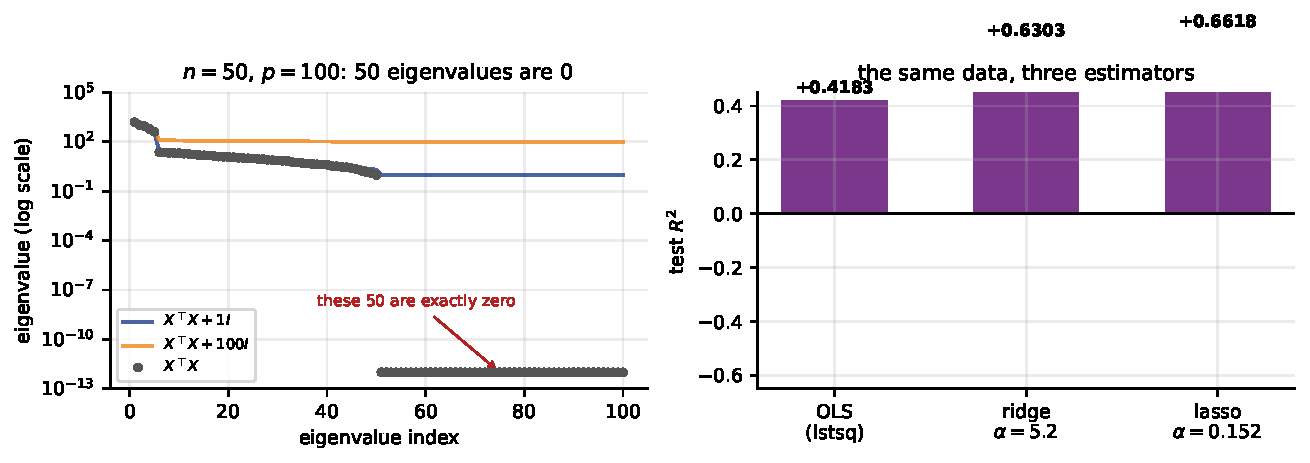
\includegraphics[width=0.90\textwidth]{pgtn.pdf}
  \end{center}
  \begin{center}\small
    Left: the eigenvalues of $X^{\!\top}\!X$ on a log scale. Fifty of the
    hundred are $0$ --- plotted on the floor of the axis because
    $\log 0$ does not exist. Adding $\lambda I$ raises the whole spectrum by
    $\lambda$. Right: what that is worth on held-out data.
  \end{center}
\end{frame}

\begin{frame}[fragile,shrink=6]{What ridge does, direction by direction (the SVD view)}
Write $X = UDV^{\!\top}$. Then the fitted values are
$X\hat\beta^{\,\mathrm{ridge}} = \sum_j u_j\,
\dfrac{d_j^2}{d_j^2 + \lambda}\, u_j^{\!\top}y$.
\begin{outblk}
diabetes, standardised: singular values of X
[42.17 25.68 23.09 20.55 17.11 16.32 15.4  13.85  5.88  1.95]
shrinkage factor d_j^2 / (d_j^2 + lambda), per direction
  lambda    d1    d2    d3    d4    d5    d6    d7    d8    d9    d10
       1  0.999 0.998 0.998 0.998 0.997 0.996 0.996 0.995 0.972 0.791
    1000  0.640 0.397 0.348 0.297 0.226 0.210 0.192 0.161 0.033 0.004
effective degrees of freedom  df(lambda) = sum d_j^2/(d_j^2+lambda):
   lambda         0   df 10.0000   lambda      1000   df  2.5087
   lambda       100   df  6.5923   lambda     10000   df  0.4042
\end{outblk}
\onslide<2->
\begin{alertblock}{Ridge shrinks the \emph{low-variance} directions hardest}
  \footnotesize At $\lambda = 1000$ the widest direction keeps $64\%$ of
  itself and the narrowest keeps $0.4\%$. Those narrow directions are exactly
  where the collinearity lives and where the estimates are least reliable.
  \textbf{$\mathrm{df}(\lambda)$ falls from $10$ to $2.5$ --- the same ten
  columns, a much smaller model.}
\end{alertblock}
\end{frame}

% =====================================================================
\section[Lasso]{Lasso}
\label{sec:lasso}

\begin{frame}[shrink=6]{Change one exponent}
  \begin{columns}[T]
    \begin{column}{0.47\textwidth}
      \begin{block}{Ridge (L2)}
        \[ \text{RSS} + \lambda \sum_{j=1}^{p} \beta_j^2 \]
        Smooth. Differentiable everywhere. Closed form.
      \end{block}
    \end{column}
    \begin{column}{0.49\textwidth}
      \begin{block}{Lasso (L1)}
        \[ \text{RSS} + \lambda \sum_{j=1}^{p} |\beta_j| \]
        Convex, but \textbf{not differentiable at $\beta_j = 0$}. No closed
        form.
      \end{block}
    \end{column}
  \end{columns}
  \vspace{0.3em}
  \begin{alertblock}{Why the derivative matters so much}
    \small $\frac{d}{d\beta}\beta^2 = 2\beta$, which is $0$ at $\beta = 0$: a
    coefficient already at zero feels \emph{no} pull from the L2 penalty, so
    there is nothing to hold it there.\\[0.3em]
    $\frac{d}{d\beta}|\beta| = \pm 1$, which does not go to zero as
    $\beta \to 0$: the L1 penalty pulls with \textbf{constant force right up
    to the origin}, so it can push a coefficient to exactly $0$ and hold it.
  \end{alertblock}
  \begin{center}\small
    \textbf{Ridge shrinks. Lasso shrinks \emph{and selects}.} That one
    sentence is the examinable content of this section.
  \end{center}
\end{frame}

\begin{frame}[shrink=8]{Why there is no matrix formula}
  Setting the gradient to zero needs a gradient. At $\beta_j = 0$ the function
  $|\beta_j|$ has none; it has a \textbf{subdifferential}, the whole interval
  $[-1, 1]$. The stationarity condition becomes
  \[
    X^{\!\top}(y - X\beta) \;=\; \lambda\,s,
    \qquad
    s_j \in
    \begin{cases}
      \{\operatorname{sign}(\beta_j)\} & \beta_j \ne 0,\\[2pt]
      [-1, 1] & \beta_j = 0 .
    \end{cases}
  \]
  \begin{block}{You cannot invert that}
    \small $s$ depends on which coefficients are zero, and which coefficients
    are zero depends on $s$. There is no matrix you can pre-multiply by ---
    \emph{unless} $X^{\!\top}\!X$ is diagonal, in which case the problem
    decouples into $p$ one-dimensional problems we can solve exactly. That
    special case is the next slide, and the general algorithm
    (\textbf{coordinate descent}: fix every coefficient but one, solve that
    one exactly, repeat) is nothing but that special case applied one
    coordinate at a time.
  \end{block}
\end{frame}

\begin{frame}[shrink=6]{By hand \#3: the orthonormal case, exactly solvable}
  Suppose $X^{\!\top}\!X = I$. Then
  $\text{RSS} = \text{const} + \sum_j\big[(\beta_j - \hat\beta_j)^2\big]$
  where $\hat\beta = X^{\!\top}y$ is the OLS answer, so the problem
  \emph{separates}:
  \[
    \min_{\beta_j}\ (\beta_j - \hat\beta_j)^2 + \lambda\,\text{pen}(\beta_j)
    \qquad\text{one $j$ at a time.}
  \]
  \begin{center}\small
  \begin{tabular}{@{}lll@{}}
    \toprule
    & \textbf{Solution} & \textbf{Behaviour}\\
    \midrule
    ridge & $\dfrac{\hat\beta_j}{1 + \lambda}$
      & every coefficient scaled by the \emph{same factor}\\[8pt]
    lasso & $\operatorname{sign}(\hat\beta_j)
      \big(|\hat\beta_j| - \tfrac{\lambda}{2}\big)_{+}$
      & every coefficient moved by the \emph{same amount}, and clipped at
        $0$\\
    \bottomrule
  \end{tabular}
  \end{center}
  \begin{block}{The second one has a name: \emph{soft thresholding}}
    \small Anything with $|\hat\beta_j| \le \lambda/2$ is set to exactly zero.
    Not ``very small''. \textbf{Zero.}
  \end{block}
\end{frame}

\begin{frame}[fragile,shrink=8]{The same four numbers, checked against the library}
The OLS coefficients are $(3,\ 1,\ -0.4,\ 0.2)$ on an orthonormal design, and
$\lambda = 1$, so the lasso threshold is $\lambda/2 = 0.5$.
\begin{outblk}
orthonormal design: X'X = I to 8.9e-16
OLS coefficients         [ 3.   1.  -0.4  0.2]
  ridge  beta_j / (1 + lambda)               [ 1.5  0.5 -0.2  0.1]
  lasso  sign(beta_j) (|beta_j| - lambda/2)+ [2.5 0.5 0.  0. ]
  exact zeros produced by lasso: 2 of 4
  Ridge(alpha=1).coef_ =         [ 1.5  0.5 -0.2  0.1]
  Lasso(alpha=1/(2n)).coef_ =    [ 2.5  0.5 0.  0. ]
\end{outblk}
\onslide<2->
\begin{alertblock}{Read the two middle rows against each other}
  \footnotesize Ridge halved all four: $3 \to 1.5$, $0.2 \to 0.1$. Lasso
  subtracted $0.5$ from all four and clipped: $3 \to 2.5$, and
  $-0.4$ and $0.2$ became \textbf{exactly zero}. \textbf{The biggest
  coefficient is punished hardest by ridge and least, proportionally, by
  lasso.}
\end{alertblock}
\onslide<3->
\begin{center}\footnotesize
  Units warning: \texttt{Ridge(alpha=a)} minimises
  $\|y-X\beta\|^2 + a\|\beta\|^2$, so $a = \lambda$; \texttt{Lasso(alpha=a)}
  minimises $\frac{1}{2n}\|y-X\beta\|^2 + a\|\beta\|_1$, so
  $\lambda = 2na$. Here $n = 200$, hence $a = 1/400$.
\end{center}
\end{frame}

\begin{frame}[shrink=8]{Drawn: two shrinkage rules}
  \begin{center}
    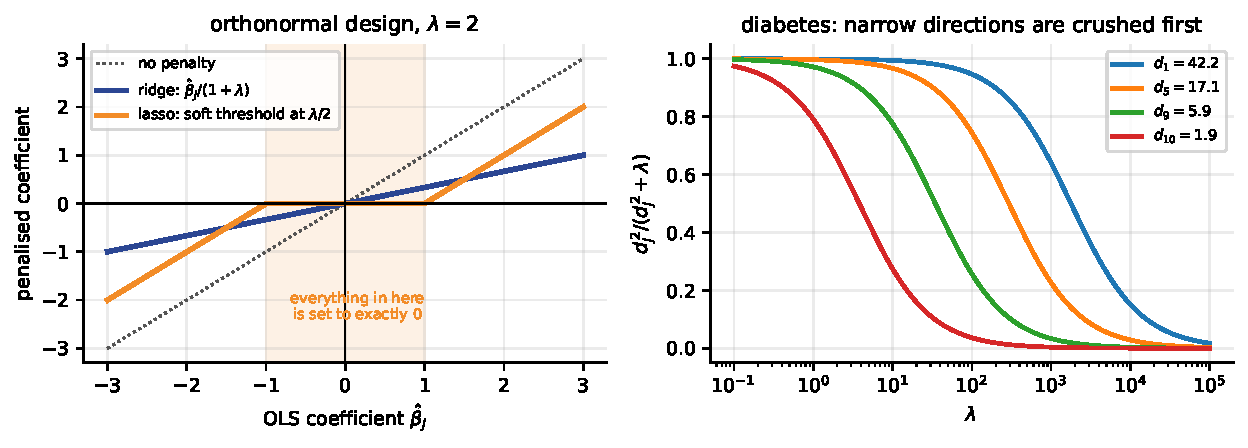
\includegraphics[width=0.88\textwidth]{shrinkage.pdf}
  \end{center}
  \begin{center}\small
    Left: ridge is a straight line through the origin with slope
    $1/(1+\lambda)$ --- it touches zero only at zero. Lasso is a straight line
    \emph{shifted}, with a flat dead zone of width $\lambda$ in the middle.
    Right: on real data, the direction with the smallest singular value is
    crushed first.
  \end{center}
\end{frame}

\begin{frame}[fragile,shrink=8]{No formula, so: twenty lines of coordinate descent}
\begin{lstlisting}
def lasso_cd(X, y, alpha, iters=500):          # (1/2n)||y-Xb||^2 + alpha|b|_1
    n, p = X.shape;  b = np.zeros(p);  r = y - X @ b
    norms = (X ** 2).sum(axis=0)
    for _ in range(iters):
        for j in range(p):
            r += X[:, j] * b[j]                          # take column j out
            rho = X[:, j] @ r / n
            b[j] = soft_threshold(rho, alpha) / (norms[j] / n)
            r -= X[:, j] * b[j]                          # put it back
    return b
\end{lstlisting}
\begin{outblk}
  alpha 2.0  my 20-line coordinate descent vs sklearn:  max |difference| 9.29e-12
     mine    [ 0.      -7.5682  24.6228  13.1778  -2.7169  0.     -10.0536  0.  23.1479  1.6904]
     sklearn [ 0.      -7.5682  24.6228  13.1778  -2.7169  0.     -10.0536  0.  23.1479  1.6904]
     exact zeros: mine 3, sklearn 3
\end{outblk}
\onslide<2->
\begin{center}\small
  Agreement to $10^{-11}$ on all ten coefficients. \textbf{The zeros are exact
  because the update \emph{assigns} zero; it does not approach it.} That is
  the entire difference from ridge, expressed as one line of code.
\end{center}
\end{frame}

\begin{frame}[shrink=6]{The geometry: a diamond has corners, a disc does not}
  \begin{columns}[T]
    \begin{column}{0.50\textwidth}
      \begin{block}{The constrained picture}
        \small The RSS contours are ellipses centred on
        $\hat\beta^{\mathrm{OLS}}$. The solution is where the smallest
        ellipse first \emph{touches} the constraint region.
      \end{block}
      \begin{block}{The two regions in two dimensions}
        \small $\|\beta\|_1 \le t$ is a \textbf{diamond}, whose four corners
        sit \emph{on the axes}.\\[0.25em]
        $\|\beta\|_2 \le s$ is a \textbf{disc}, which is smooth everywhere and
        has no distinguished points at all.
      \end{block}
    \end{column}
    \begin{column}{0.46\textwidth}
      \begin{alertblock}{Why corners produce zeros}
        \small A corner is where the boundary has a \emph{kink}. An ellipse
        arriving from a generic direction will meet a kink before it meets any
        smooth part --- and a corner of the diamond has
        $\beta_j = 0$ for every $j$ but one.\\[0.3em]
        A disc has no kink, so the touching point is generically in the
        interior of a quadrant: \textbf{all coefficients non-zero}.
      \end{alertblock}
    \end{column}
  \end{columns}
  \vspace{0.2em}
  \begin{center}\small
    In $p$ dimensions the L1 ball has corners, edges and faces of every
    dimension from $0$ to $p-1$ --- a whole hierarchy of ways to be sparse.
  \end{center}
\end{frame}

\begin{frame}[shrink=8]{Drawn: the same budget, two answers}
  \begin{center}
    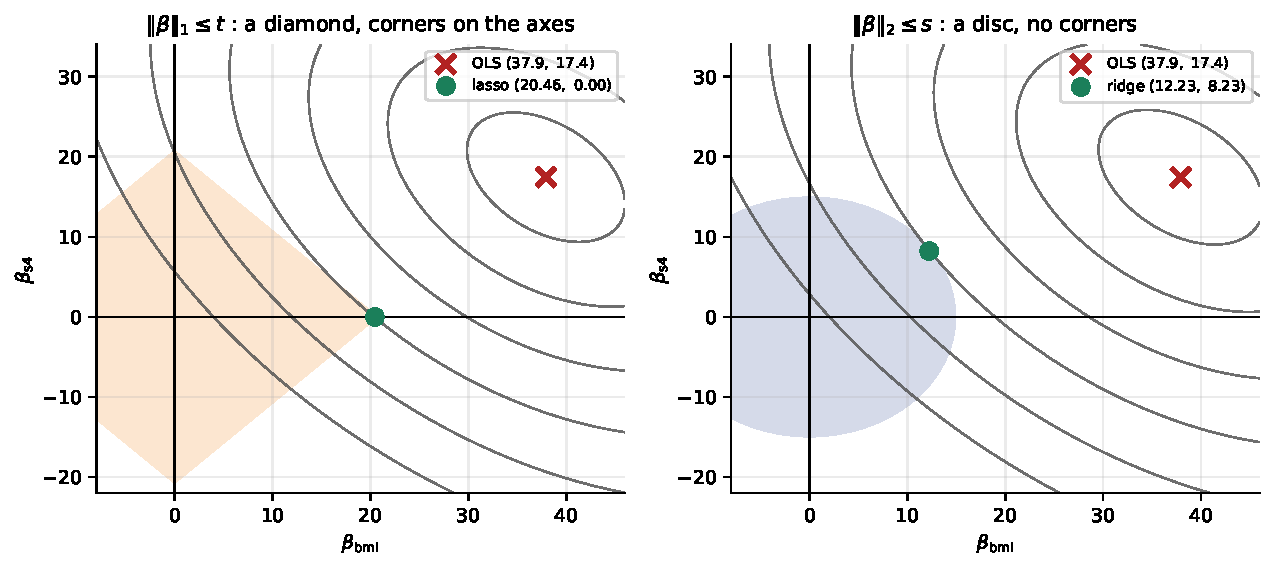
\includegraphics[width=0.86\textwidth]{geometry.pdf}
  \end{center}
  \begin{center}\small
    Two standardised diabetes columns. OLS is at $(37.9, 17.4)$. Constrain to
    $\|\beta\|_1 \le 20.46$ and the answer is the corner
    $(20.46,\ \mathbf{0.00})$; give ridge \emph{the same L1 budget} and it
    answers $(12.23,\ 8.23)$. \textbf{Same budget, and one of them deletes a
    predictor.}
  \end{center}
\end{frame}

% =====================================================================
\section[Paths]{Coefficient paths}
\label{sec:paths}

\begin{frame}[fragile,shrink=8]{Predict first \#3}
Standardised diabetes, ten features. Sweep $\alpha$ from tiny to large under
both penalties.

\begin{center}
  \textbf{At $\alpha = 100$, how many ridge coefficients are exactly zero?
  And how many lasso coefficients, at the $\alpha$ that gives the same amount
  of shrinkage?}
\end{center}
\vspace{0.2em}
\onslide<2->
\begin{outblk}
  alpha        ridge nonzero  min|coef|   lasso nonzero  kept
  ridge a=0.01    lasso a=0.000    10        0.4756      10   age, sex, bmi, bp, s1, s2, s3, s4, s5, s6
  ridge a=10.00   lasso a=0.100    10        0.2579       9   age, sex, bmi, bp, s1, s2, s4, s5, s6
  ridge a=50.00   lasso a=0.500    10        0.1070       8   sex, bmi, bp, s1, s3, s4, s5, s6
  ridge a=100.00  lasso a=1.000    10        0.4361       7   sex, bmi, bp, s1, s3, s5, s6
ridge never returns an exact zero: smallest |coef| over the whole grid
   1.455e-03 at alpha up to 1e6 -- small, never 0
\end{outblk}
\onslide<3->
\begin{alertblock}{Ridge: ten, ten, ten, ten. For ever.}
  \footnotesize Even at $\alpha = 10^{6}$, where the coefficients are of order
  $10^{-3}$, none of them is zero. \textbf{Ridge gives you a smaller model;
  lasso gives you a shorter one.} If the deliverable is ``which five
  measurements do we actually need'', only one of those helps.
\end{alertblock}
\end{frame}

\begin{frame}[shrink=8]{Drawn: the figure this lecture is for}
  \begin{center}
    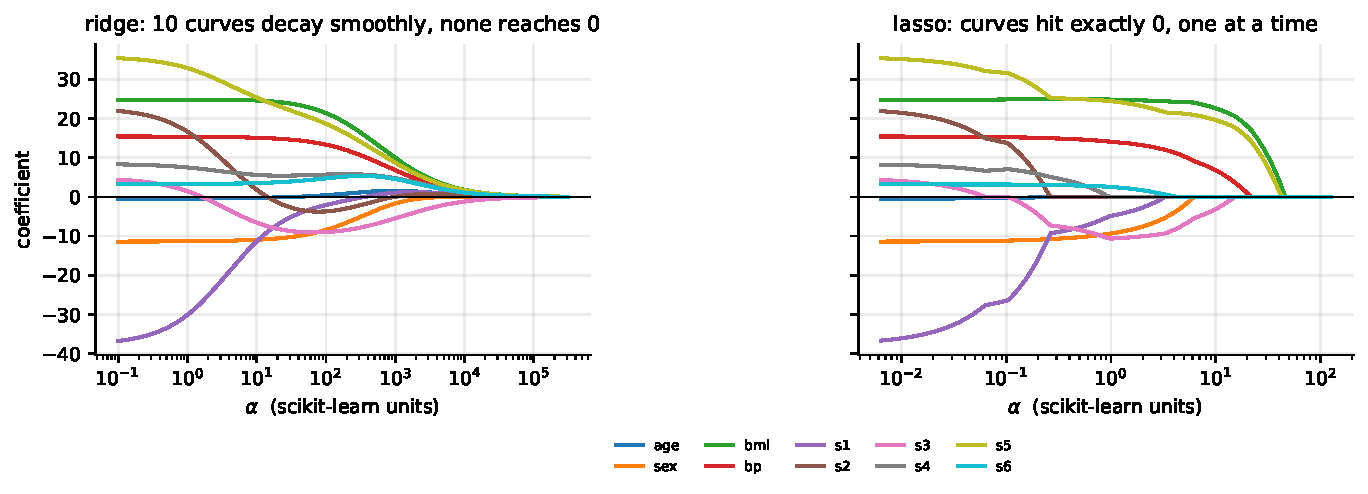
\includegraphics[width=0.98\textwidth]{paths.pdf}
  \end{center}
  \begin{center}\small
    Ten coefficients, one colour each, as $\alpha$ sweeps six orders of
    magnitude. \textbf{Left: ten curves glide towards the axis and never
    arrive. Right: they land on it, one at a time, and stay.}
  \end{center}
\end{frame}

\begin{frame}[fragile,shrink=8]{The order of deletion is the ranking}
\begin{outblk}
as alpha RISES, lasso coefficients hit exactly zero in this order:
    1. age  leaves at alpha =  0.2473        6. sex  leaves at alpha =  6.3339
    2. s2   leaves at alpha =  0.2641        7. s3   leaves at alpha = 15.3382
    3. s4   leaves at alpha =  0.9790        8. bmi  never
    4. s1   leaves at alpha =  3.2897        9. bp   never
    5. s6   leaves at alpha =  4.2753       10. s5   never
   alpha   5.00   nonzero  5   R2 on the training rows +0.4892
   alpha   0.05   nonzero 10   R2 on the training rows +0.5176
\end{outblk}
\onslide<2->
\begin{center}\small
  \textbf{Half the features and $94.5\%$ of the training $R^2$.} The last
  three standing --- body mass index, blood pressure and \texttt{s5} --- are
  the three a clinician would have named.
\end{center}
\onslide<3->
\begin{outblk}
the count is not perfectly monotone, and that is real, not a bug:
   alpha  0.15  nonzero 10   coefficient on s3 -2.13916
   alpha  0.10  nonzero  9   coefficient on s3 -0.00000
   alpha  0.05  nonzero 10   coefficient on s3 +0.95082
\end{outblk}
\end{frame}

% =====================================================================
\section[Scaling]{Scaling is not optional}
\label{sec:scale}

\begin{frame}[fragile,shrink=10]{Where the penalty budget actually goes}
$\lambda\sum_j\beta_j^2$ adds up $p$ numbers as if they were commensurable.
\textbf{They are not.} Multiply column $j$ by $c$: under OLS $\beta_j$ becomes
$\beta_j/c$ and every prediction is unchanged; under ridge its penalty
contribution becomes $\lambda\beta_j^2/c^2$. So a column recorded in
\emph{large} numbers is effectively unregularised, and one recorded in
\emph{small} numbers gets crushed.

\texttt{load\_diabetes(scaled=False)}, ridge with $\alpha = 100$.
\begin{outblk}
     name    column sd    ridge coef   lambda*coef^2   share of penalty
     age       13.295       -0.1608            2.59         0.0002
     sex        0.500       -7.2829         5304.01         0.3758
     bmi        4.480        6.7139         4507.62         0.3194
     bp        13.846        0.9030           81.55         0.0058
     s1        34.433        1.3138          172.62         0.0122
     s5         0.539        5.7095         3259.84         0.2310
     s6        12.321        0.1567            2.46         0.0002
\end{outblk}
\onslide<2->
\begin{alertblock}{Three narrow columns pay $93\%$ of the penalty}
  \footnotesize \texttt{sex} ($\mathrm{sd}\,0.50$), \texttt{bmi}
  ($4.48$) and \texttt{s5} ($0.54$) together take
  $0.3758 + 0.3194 + 0.2310 = \mathbf{0.9262}$ of the budget.
  \texttt{age} and \texttt{s6}, whose standard deviations are $13$, pay
  $0.0002$ each. \textbf{The penalty is being spent on the columns with the
  smallest numbers, not the ones with the least evidence.}
\end{alertblock}
\end{frame}

\begin{frame}[fragile,shrink=8]{Predict first \#4}
Take \texttt{bmi} and divide it by $100$ --- report it as a fraction rather
than in kg per square metre. Nothing else changes; the information is
identical.

\begin{center}
  \textbf{What happens to the OLS fit? What happens to the ridge fit?}
\end{center}
\vspace{0.2em}
\onslide<2->
\begin{outblk}
     OLS   coef on bmi       6.2458 ->     624.5825   ratio   100.0000
     OLS   test R2     +0.392899 -> +0.392899   (the same fit)
     ridge coef on bmi       6.7139 ->       2.8018   ratio     0.4173
     ridge test R2     +0.358505 -> +0.309806   (a DIFFERENT model)
     bmi's share of the ridge penalty  0.3194 -> 0.0410
     max |prediction difference|, OLS   8.697e-12
     max |prediction difference|, ridge 71.0177
\end{outblk}
\onslide<3->
\begin{alertblock}{$8.7\times10^{-12}$ against $71.0$}
  \footnotesize OLS is \textbf{equivariant}: the coefficient scales by exactly
  $100$ and the predictions do not move by a picogram. Ridge is not: the
  coefficient moves by a factor of $0.42$, and predictions on the same
  patients shift by up to $71$ units of a target that ranges from $25$ to
  $346$. \textbf{A change of unit changed the model.}
\end{alertblock}
\end{frame}

\begin{frame}[fragile,shrink=8]{And under lasso, a change of unit deletes a predictor}
\begin{outblk}
  the same unit change under lasso, which also selects:
     alpha 1  kg/m^2 units: kept 9  age sex bmi bp s1 s2 s3 s5 s6
     alpha 1  bmi/100    : kept 7  age sex bp s2 s3 s5 s6
\end{outblk}
\onslide<2->
\begin{center}\small
  \textbf{\texttt{bmi} is gone.} The single most predictive variable in the
  dataset was removed from the model, not because the evidence changed but
  because somebody chose to divide it by a hundred. \texttt{s1} went with it.
\end{center}
\onslide<3->
\begin{outblk}
  ridge across a grid of alpha, raw units against standardised:
        alpha     raw test R2   standardised test R2
              1      +0.3919            +0.3916
            100      +0.3585            +0.4073
          10000      +0.3539            +0.0699
\end{outblk}
\begin{center}\small
  Standardised, the best available $\alpha$ reaches $0.4073$; on raw units the
  curve never gets above $0.3919$, and it gets there by turning the penalty
  \emph{off}.
\end{center}
\end{frame}

\begin{frame}[shrink=8]{Drawn: two panels, one rule}
  \begin{center}
    
\includegraphics[width=0.94\textwidth]{scaling.pdf}
  \end{center}
  \begin{center}\small
    Left: the share of $\sum_j\beta_j^2$ each column consumes, raw against
    standardised. Right: test $R^2$ against $\alpha$. \textbf{The orange curve
    is not a worse version of the purple one --- it is a different
    experiment, in which $\alpha$ means something else.}
  \end{center}
\end{frame}

\begin{frame}[fragile,shrink=8]{The intercept is not penalised, and here is the proof}
Shift every target up by $500$ and refit.
\begin{outblk}
ridge with alpha = 100, then the same fit with y shifted up by 500
  intercept       152.1197 ->     652.1197   difference 500.0000
  max |coefficient difference|  1.288e-14
  mean of y = 152.1197, intercept of the unshifted fit = 152.1197
\end{outblk}
\onslide<2->
\begin{outblk}
what happens if you DO penalise it -- fit_intercept=False on uncentred y:
   alpha        1   with intercept R2 +0.3916   without -3.8362
   alpha      100   with intercept R2 +0.4073   without -3.8990
Ridge(alpha=1e12): intercept 152.1197, max|coef| 1.512e-08, prediction 152.1197
\end{outblk}
\onslide<3->
\begin{alertblock}{Two things to take away}
  \footnotesize The intercept absorbed the shift \emph{exactly}
  ($+500.0000$) and no coefficient moved by more than $10^{-14}$. And it
  equals $\bar y$. Penalise it instead --- \texttt{fit\_intercept=False} on
  data whose mean is $152$ --- and $R^2$ goes to $\mathbf{-3.84}$.
  \textbf{As $\lambda \to \infty$ ridge must predict a constant, and the right
  constant is $\bar y$.}
\end{alertblock}
\end{frame}

% =====================================================================
\section[Choosing $\lambda$]{Choosing $\lambda$ by cross-validation}
\label{sec:cv}

\begin{frame}[fragile,shrink=11]{The U-curve, the minimum and the 1-SE choice}
Hold out a test set and do not look at it. On the training rows take a
\emph{logarithmic} grid of $\lambda$, run $k$-fold cross-validation at each,
and record the mean validation error \textbf{and its standard error}. Then
choose --- two answers are defensible. \textbf{The minimum:} lowest mean CV
error. \textbf{The one-standard-error rule:} the \emph{largest} $\lambda$
whose mean is still within one standard error of the minimum, because the
curve is flat near the bottom and estimated with noise.
\begin{outblk}
RIDGE, 5-fold CV on the training rows, 60 alphas from 1e-2 to 1e4
  minimum        alpha   22.6951   CV MSE  3050.64   se 219.00
  1-SE threshold                    CV MSE  3269.64
  1-SE choice    alpha  147.7378   CV MSE  3213.05
     alpha   22.6951  test R2 +0.3971  test MSE  3075.84  ||beta||   41.799
     alpha  147.7378  test R2 +0.4049  test MSE  3035.86  ||beta||   32.073
  for comparison, OLS (alpha = 0): test R2 +0.3929  test MSE  3097.12
\end{outblk}
\onslide<2->
\begin{outblk}
LASSO, same folds
  minimum        alpha    0.9769   test R2 +0.3889  nonzero  8
  1-SE choice    alpha    9.6926   test R2 +0.3616  nonzero  4   bmi, bp, s3, s5
\end{outblk}
\onslide<3->
\begin{alertblock}{The 1-SE rule was the better choice for ridge here}
  \footnotesize $\alpha = 147.7$ beat $\alpha = 22.7$ on the test set
  ($0.4049$ against $0.3971$) with a coefficient vector $23\%$ shorter --- and
  both beat OLS. For lasso it cost $0.027$ of $R^2$ and bought a model with
  \textbf{four features instead of eight}. That is a trade you may want.
\end{alertblock}
\end{frame}

\begin{frame}[shrink=8]{Drawn: read the shape, not just the minimum}
  \begin{center}
    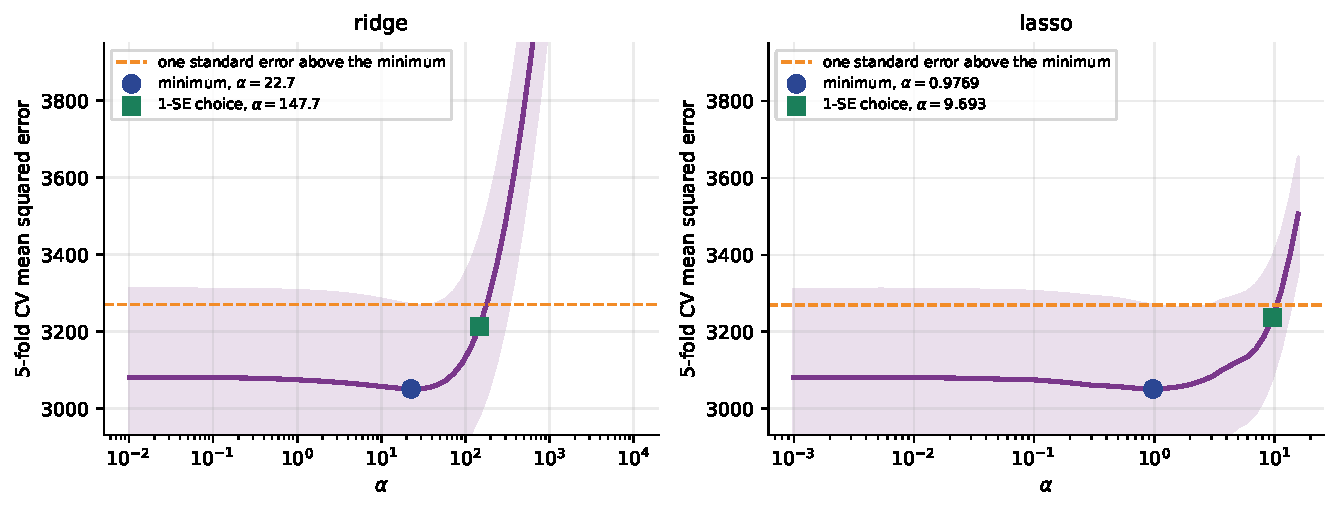
\includegraphics[width=0.94\textwidth]{cvcurve.pdf}
  \end{center}
  \begin{center}\small
    The shaded band is $\pm$ one standard error across the five folds. Both
    curves are \textbf{flat for three orders of magnitude} and then climb
    steeply. The dashed line is the 1-SE threshold; the square is the largest
    $\alpha$ still under it.
  \end{center}
\end{frame}

% =====================================================================
\section[Bias--variance]{The trade being made}
\label{sec:bv}

\begin{frame}[shrink=6]{Ridge is biased. On purpose.}
  Take $X^{\!\top}\!X = I$ so the algebra is clean, and write
  $\hat\beta^{R} = \hat\beta^{\mathrm{OLS}}/(1+\lambda)$. Then
  \[
    \mathbb{E}[\hat\beta^{R}] = \frac{\beta}{1+\lambda},
    \qquad
    \operatorname{bias} = -\frac{\lambda}{1+\lambda}\beta,
    \qquad
    \operatorname{Var}(\hat\beta^{R}) = \frac{\sigma^2}{(1+\lambda)^2} I .
  \]
  \begin{block}{So the total squared error is}
    \[
      \mathrm{MSE}(\lambda)
      = \underbrace{\frac{\lambda^2 \|\beta\|^2}{(1+\lambda)^2}}_{\text{bias}^2,\ \uparrow}
      + \underbrace{\frac{\sigma^2 p}{(1+\lambda)^2}}_{\text{variance},\ \downarrow}
      = \frac{\lambda^2\|\beta\|^2 + \sigma^2 p}{(1+\lambda)^2} .
    \]
  \end{block}
  \begin{alertblock}{Differentiate and something remarkable falls out}
    \small
    $\mathrm{MSE}'(\lambda) = \dfrac{2(\lambda\|\beta\|^2 - \sigma^2p)}{(1+\lambda)^3}$,
    so the minimum is at
    $\boxed{\lambda^\star = \sigma^2 p / \|\beta\|^2}$ --- and
    $\mathrm{MSE}'(0) = -2\sigma^2 p < 0$. \textbf{$\lambda = 0$ is never
    optimal. There is always a positive $\lambda$ that beats least squares.}
  \end{alertblock}
\end{frame}

\begin{frame}[fragile,shrink=8]{Measured, on $400$ training sets}
$p = 25$, $n = 40$, $\sigma = 2$. Redraw the training data $400$ times, fit
ridge at each $\lambda$, and decompose the error on $500$ fixed test points.
\begin{outblk}
  lambda      bias^2   variance   noise   expected test MSE
      0.010    0.0226     6.9702    4.00     10.9928
      1.805    0.1585     4.3535    4.00      8.5119
      4.781    0.6766     3.1703    4.00      7.8469
    170.125   12.1011     0.3214    4.00     16.4225
   3162.278   17.2243     0.0022    4.00     21.2265
  variance removed 3.7998, bias added 0.6540, net gain 3.1459
  the net gain is 45.0% of the reducible error (10.9928 - 4.00 = 6.9928)
  check: bias^2 + variance reproduces the measured squared error to 7.11e-15
  theory says the best lambda is sigma^2 p / ||beta||^2 = 5.4298
  measured optimum 4.781
\end{outblk}
\onslide<2->
\begin{alertblock}{$0.65$ of bias bought $3.80$ of variance}
  \footnotesize A net saving of $\mathbf{3.15}$, which is $45\%$ of the
  reducible error. And the closed form landed in the right place without
  being exact: $\lambda^\star = 5.43$ against a measured $4.78$, $14\%$
  high, because $X^{\top}X$ here is Wishart and not $I$.
  \textbf{Regularization is not a trick; it is an accounting identity you can
  compute in advance.}
\end{alertblock}
\end{frame}

\begin{frame}[shrink=8]{Drawn: the two curves that cross}
  \begin{center}
    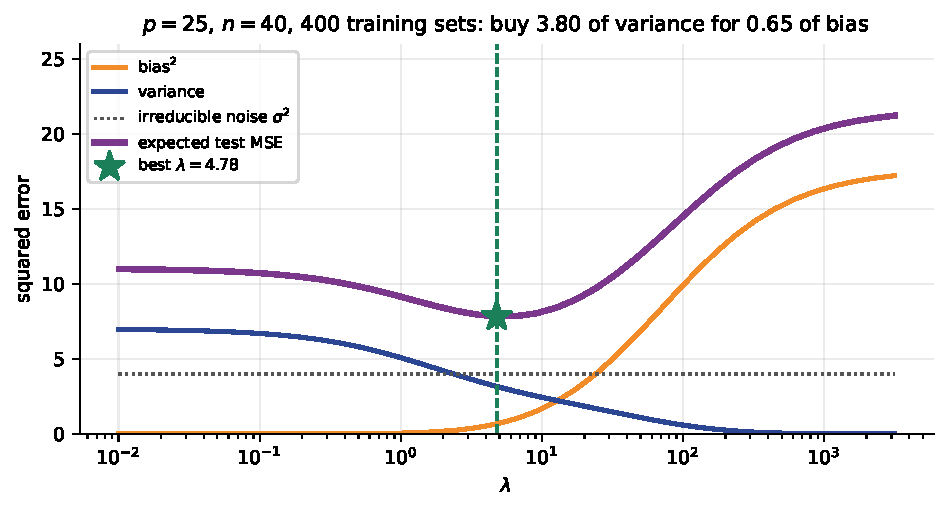
\includegraphics[width=0.72\textwidth]{biasvar.pdf}
  \end{center}
  \begin{center}\small
    Bias$^2$ climbs from nothing, variance falls to nothing, and their sum has
    a minimum strictly to the right of zero. The dotted line is $\sigma^2 = 4$,
    the part no model can remove. \textbf{The right-hand end of the purple
    curve is the constant model; the left-hand end is least squares.}
  \end{center}
\end{frame}

% =====================================================================
\section[Elastic net]{Elastic net}
\label{sec:enet}

\begin{frame}[shrink=6]{Why a third penalty exists}
  \[
    \text{RSS} \;+\; \lambda\Big[\,\rho\sum_j |\beta_j|
      \;+\; (1-\rho)\sum_j \beta_j^2\,\Big],
    \qquad \rho \in [0, 1] .
  \]
  \small In scikit-learn: \texttt{ElasticNet(alpha=$\lambda$,
  l1\_ratio=$\rho$)}. $\rho = 1$ is lasso, $\rho = 0$ is ridge.
  \vspace{0.3em}
  \begin{columns}[T]
    \begin{column}{0.48\textwidth}
      \begin{alertblock}{The problem it fixes}
        \small Given a group of strongly correlated predictors that all carry
        the signal, \textbf{lasso picks one and discards the rest} --- and
        which one it picks is close to arbitrary. Resample the data and the
        answer changes.
      \end{alertblock}
    \end{column}
    \begin{column}{0.48\textwidth}
      \begin{block}{Why the L2 term fixes it}
        \small $\sum\beta_j^2$ is minimised, for a fixed sum, by spreading the
        weight \emph{evenly}. So the L2 part wants the group to share; the L1
        part still lets the whole group be dropped together. This is called
        the \textbf{grouping effect}.
      \end{block}
    \end{column}
  \end{columns}
  \begin{center}\small
    It also lets you select more than $n$ variables when $p > n$, which lasso
    cannot.
  \end{center}
\end{frame}

\begin{frame}[fragile,shrink=11]{Three near-copies of one signal, and their stability}
$x_1, x_2, x_3$ are the same latent variable plus a little noise (pairwise
correlation $0.9971$); seven pure-noise columns follow.
\begin{outblk}
  lasso       coefficients on the group [2.1943 0.3251 0.0565]
  elastic net coefficients on the group [0.8844 0.8606 0.8602]
  ridge       coefficients on the group [0.806  0.7954 0.7973]
stability: refit on 30 bootstrap resamples, count how often each is kept
  lasso       kept x1 29/30, x2 13/30, x3 21/30
  elastic net kept x1 30/30, x2 30/30, x3 30/30
prediction on 400 fresh rows:  lasso +0.9609  elastic net +0.9636  ridge +0.9435
\end{outblk}
\onslide<2->
  \begin{center}
    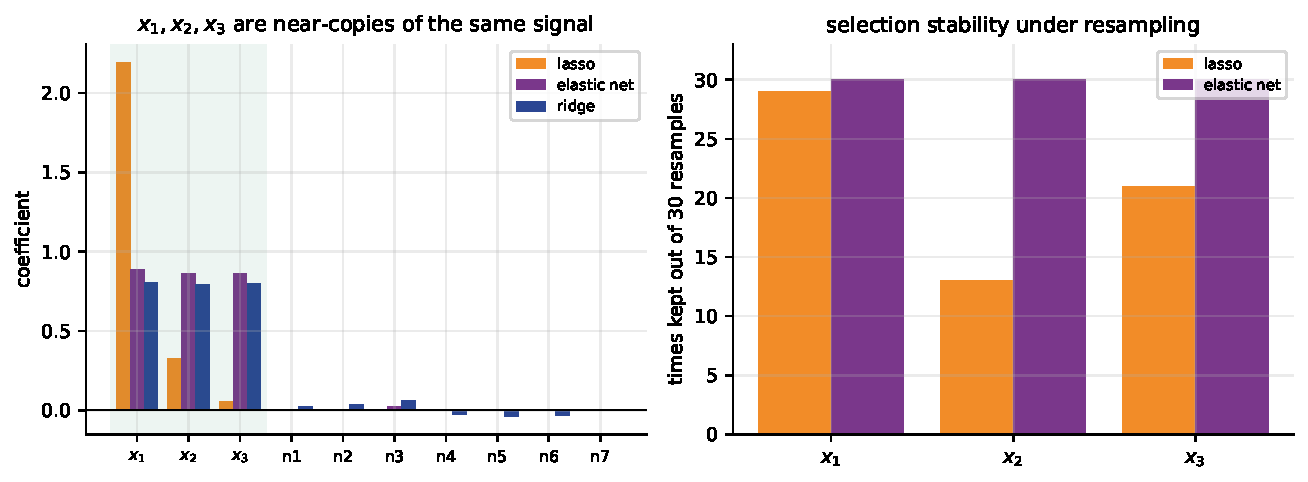
\includegraphics[width=0.66\textwidth]{elasticnet.pdf}
  \end{center}
\onslide<3->
\begin{alertblock}{$29/30$, $13/30$, $21/30$ against $30/30$, $30/30$, $30/30$}
  \footnotesize The three columns are indistinguishable, and lasso ranks
  them anyway: $x_1$ survives $29$ resamples, $x_3$ survives $21$, $x_2$ only
  $13$. \textbf{If you report ``the lasso selected $x_1$'' you are reporting
  a coin flip.} Elastic net kept all three every time, and predicted
  marginally better. \textbf{Report a selection with its stability, or do not
  report it.}
\end{alertblock}
\end{frame}

% =====================================================================
\section{Summary}
\label{sec:summary}

\begin{frame}[fragile,shrink=6]{All four on the same data, end to end}
\begin{lstlisting}
pipe = make_pipeline(StandardScaler(), RidgeCV(alphas=np.logspace(-2, 4, 60)))
pipe.fit(X_train, y_train);  pipe.score(X_test, y_test)
\end{lstlisting}
\begin{outblk}
diabetes, 70/30 split, everything inside a Pipeline
  model              train R2   test R2   nonzero of 10
  OLS                 +0.5539   +0.3929        10
  Ridge, CV alpha     +0.5505   +0.3989        10
  Lasso, CV alpha     +0.5517   +0.3889         8
  ElasticNet 0.5      +0.5529   +0.3917        10
\end{outblk}
\onslide<2->
\begin{alertblock}{Report this honestly}
  \footnotesize On a $442\times10$ problem with no collinearity crisis,
  regularization is worth \textbf{six thousandths of $R^2$}. That is the
  truthful result and you should say so. Its value here is not accuracy: it
  is that lasso answered the question ``which eight?''. \textbf{Go back to
  the $n=50$, $p=100$ table for the case where it lifts test $R^2$ from
  $0.4183$ to $0.6303$.}
\end{alertblock}
\end{frame}

\begin{frame}[shrink=16]{Summary --- twelve lines}
  \begin{enumerate}\small
    \item Regularization means minimising
      $\text{loss} + \lambda\,\text{pen}(\beta)$. $\lambda$ is not fitted; it
      is chosen by cross-validation.
    \item Ridge has a closed form,
      $\hat\beta = (X^{\!\top}\!X + \lambda I)^{-1}X^{\!\top}y$, derived in
      four lines from $\nabla J = 0$.
    \item $X^{\!\top}\!X + \lambda I$ is positive definite for every
      $\lambda>0$, because
      $v^{\!\top}(X^{\!\top}\!X+\lambda I)v = \|Xv\|^2 + \lambda\|v\|^2$.
      \textbf{Ridge exists where OLS does not.} On a perfectly collinear
      $X$, $\det(X^{\!\top}\!X) = 0$ and \texttt{inv} raises; add $\lambda=1$
      and the determinant is $71$.
    \item At $p>n$, \texttt{LinearRegression} does not fail --- it silently
      returns the minimum-norm solution, which is ridge at $\lambda\to 0$
      (agreeing to $5.9\times10^{-12}$).
    \item By hand: $x=(1,2,2)$, $y=(2,3,5)$ gives
      $\hat\beta = 18/(9+\lambda)$, so $2.0 \to 1.8 \to 1.0$ at
      $\lambda = 0, 1, 9$; \texttt{Ridge} reproduces all four to four
      decimals.
    \item In the SVD basis, ridge multiplies direction $j$ by
      $d_j^2/(d_j^2+\lambda)$ --- the \emph{narrow} directions are crushed
      first. On diabetes, $\mathrm{df}(\lambda)$ falls $10 \to 2.51$ at
      $\lambda = 1000$.
    \item Lasso has no closed form, because $|\beta|$ has no derivative at
      $0$. On an orthonormal design it is soft thresholding, and
      $(3, 1, -0.4, 0.2)$ becomes $(2.5, 0.5, 0, 0)$ --- \textbf{two exact
      zeros} --- where ridge gives $(1.5, 0.5, -0.2, 0.1)$.
    \item Geometrically the L1 ball is a diamond with corners \emph{on the
      axes}; the L2 ball has none. At the same L1 budget, lasso answered
      $(20.46, 0)$ and ridge $(12.23, 8.23)$.
    \item Scaling is not optional: three narrow raw columns took $92.6\%$ of
      the ridge penalty, and dividing \texttt{bmi} by $100$ moved OLS
      predictions by $8.7\times10^{-12}$ and ridge predictions by
      $\mathbf{71.0}$ --- and made lasso \textbf{delete \texttt{bmi}}.
    \item The intercept is not penalised: shifting $y$ by $500$ moved the
      intercept by exactly $500.0000$ and no coefficient by more than
      $1.3\times10^{-14}$. Penalise it and $R^2 = -3.84$.
    \item Cross-validation gave ridge $\alpha = 22.7$ (test $R^2\ 0.3971$) and
      the 1-SE rule $\alpha = 147.7$ (test $R^2\ \mathbf{0.4049}$); lasso's
      1-SE choice kept \textbf{four features of ten}.
    \item The trade, measured: $\lambda^\star = 4.78$ added $0.65$ of
      bias$^2$ and removed $3.80$ of variance, a net gain of $3.15$ --- and
      the closed form $\sigma^2p/\|\beta\|^2 = 5.43$ found the same place.
      \textbf{$\lambda = 0$ is never optimal.}
  \end{enumerate}
\end{frame}

\begin{frame}[shrink=4]{Unit V ends here}
  \begin{columns}[T]
    \begin{column}{0.48\textwidth}
      \begin{block}{Read}
        \texttt{notes.pdf} --- the full derivation, the subdifferential
        argument for the lasso, the bias--variance algebra, and
        \textbf{10 practice questions with worked solutions}.
      \end{block}
      \begin{block}{Do}
        Questions 2, 4 and 7. Question 2 is the ridge closed form on a
        $2\times2$ matrix by hand; question 7 is soft thresholding; question
        4 is the invertibility proof.
      \end{block}
    \end{column}
    \begin{column}{0.48\textwidth}
      \begin{exampleblock}{What Unit V built}
        Least squares, maximum likelihood and $R^2$; over-fitting and how to
        detect it; logistic regression; multiple regression and its
        pathologies; and now the one dial that controls all of them.
      \end{exampleblock}
      \begin{alertblock}{A habit to start now}
        Never write \texttt{Ridge()} or \texttt{Lasso()} outside a
        \texttt{Pipeline} that begins with \texttt{StandardScaler}, and never
        report a coefficient without saying which $\lambda$ produced it.
      \end{alertblock}
    \end{column}
  \end{columns}
  \begin{center}
    \small Materials: \texttt{\AMLRepoURL}
  \end{center}
  \slidesources{\AMLUnitVSources}
\end{frame}

\end{document}
